\chapter{本科毕业论文文献综述}
%字数要求3000字
%包括国内外现状、研究方向、进展情况、存在问题、参考依据

% 以game synchronization为中心(要不要加一个cheating avoidance?)
% (1)描述传统网络上同步算法如何 (参考已有文献综述)
% (2)描述ndn中同步算法发展到什么阶段
% (3)描述ndn的兄弟网络上同步算法发展到什么阶段(查找一下资料)

% 总的思路是说,首先同步是很重要的,其次同步的内容是很多的(包括结构和算法),再次NDN可以使P2P结构发挥很大优势,最后NDN目前对游戏的支持尚不多,尤其在同步这一块比较薄弱。说说其它的网络陪衬一番。
% 8月13日,若能在今天把这篇文章搞定,多好啊!

% 把CCN用于游戏中的好处:
% - 可以实现P2P架构,减短latency,增强robustness
% - 降低对带宽的要求,提升信息分享效率:每分数据至多走过一个链接一次,每个节点可以从离它最近的地方取到数据
%
% 不足:
% - P2P的安全问题尚未解决
% - P2P的同步机制比C/S复杂
% ————这是从游戏的角度说,游戏需要CCN,这个应该写在第一部分里面

% 从CCN的角度出发,CCN更需要游戏,因为没有任何一个网络不需要游戏的,因此综述里应该写各种不同的网络对游戏的支持(这样的话反倒应该看看那篇很宽泛的文章)——侧重于同步机制

% 一些宏定义
\newcommand{\csa}{客户~\slash~服务器架构}
\newcommand{\pa}{对等体架构}
\newcommand{\da}{分布式架构}
\newcommand{\ma}{镜像服务器架构}
\newcommand{\ioc}{I{\slash}O\_C}
\newcommand{\gss}{GSS}


\heiti
标题

\songti
不同网络中的多玩家网游同步机制

\heiti
摘要

\songti
最后写

\section{引言}
% 200字
% 任何一个网络设计师都不会忘记网络游戏,也不会忘记同步机制。
% 一句话介绍同步。
% 同步是很重要的
% 后续章节介绍
任何一个网络设计师都明白游戏对网络的重要性,也明白同步机制对于游戏的重要性。同步机制是保障游戏一致性(Consistency)的基本方法,而一致性是游戏得以公平、顺利开展的必要条件,是影响可玩度的一个重要因素。因此游戏所处的网络提供的服务和游戏所采用的同步机制常常可以影响一个游戏的命运。

在游戏产业发达的今天,网络游戏的开发者和设计者们已经积累了大量~IP~网络上的同步经验。然而随着新兴的数据命名网络的出现,游戏同步领域又产生了新的变化。

本文介绍了传统网络(以~IP~网络为代表)和新兴的数据命名网络(以~CCN~为代表)中的同步机制,综述了已有方法、发展状况和存在问题。~\ref{notion}~中介绍了网络游戏领域与同步相关的定义和标准,~\ref{traditional}~中介绍了传统~IP~网络中的经典同步机制,~\ref{innovative}~中介绍了新兴数据命名网络中的同步机制。


%============================%

\section{网络游戏与同步}
\label{notion}
% 同步的概念,
% 目标,是保持一致性 consistency
% 而 consistency,safety 的定义是有的
% 分类,分为asset, state吗?
% 同步与consistency, responsiveness有什么关系?
本节介绍了网络游戏的基本架构(\ref{archi})和游戏架构须提供的基本服务(\ref{service})。在~\ref{def}~中给出了同步和一致性的基本定义。


%-------------------------------------------------%
\subsection{游戏架构}
% 400字
\label{archi}

多人在线游戏中的玩家是分散的,为此游戏设计者和网络工程师设计了不同的拓扑结构(或称游戏架构)来适应性地为分散的用户提供服务。这些拓扑结构可以分为三类:
\begin{itemize}
\item Client {\slash} Server Architecture~\csa
\item P2P Architecture~\pa
\item Distributed Architecture~\da
\end{itemize}

对这三种结构的具体描述见下文。这里需要概括的是:不论游戏采用哪种拓扑结构,它都由两类实体组成——输入输出控制实体(I{\slash}O Client Control Entity,~简称~\ioc)和游戏状态服务器实体(Game State Server Entity,~简称~\gss)~\cite{Ferretti2005}。

\ioc~通常是一个客户端软件,负责输入输出,对~\gss~收发事件(event)和图形渲染工作。~\ioc~可以看做游戏场景中一个或多个虚拟实体的拥有者,负责更新它们的属性(attribute)~\cite{hla}。~\gss~通常负责维护游戏状态。
\renewcommand\baselinestretch{1} %调一下脚注行间距
\footnote{一个网络游戏的游戏状态指该虚拟世界和这个世界中所有角色的状态的总和。}


% . . . . . . . . . . . . . . . . . . . . . . . . . . . . . . . . %
\subsubsection{\csa} 
% 客户服务器架构  好处与缺点

{\csa}是商业界采用得最多的一种架构。~Quake \cite{quake}, Ultima Online \cite{ultima}~等游戏都采用此架构。

{\csa}只有一个中央服务器,属于~\gss~类实体;有许多客户端,属于~\ioc~类实体。~\gss~负责维护游戏状态,~\ioc~产生的所有事件都要发送到~\gss~进行运算;随后~\gss~将新的游戏状态发送给所有~\ioc。(如图~\ref{CS})

\begin{figure}[htbp]
\begin{center}
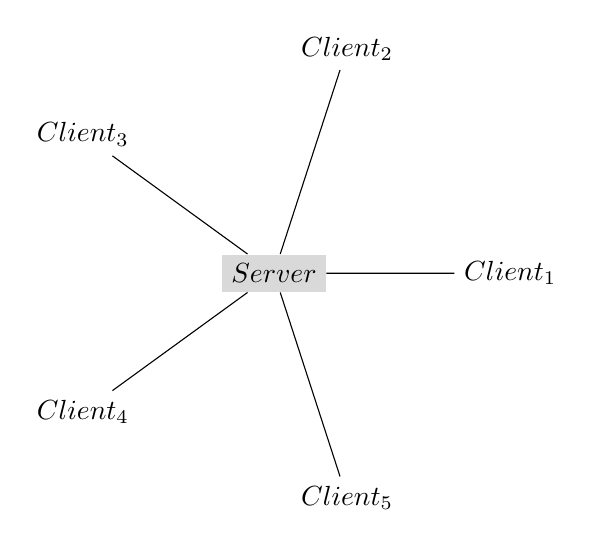
\begin{tikzpicture} [scale=1, transform shape]
%\tikzstyle{every node}=[draw,shape=circle];
\node [fill = gray!30] (v0) at (0:0) {$Server$};
\node (v1) at ( 0:3) {$Client_1$};
\node (v2) at ( 72:3) {$Client_2$};
\node (v3) at (2*72:3) {$Client_3$};
\node (v4) at (3*72:3) {$Client_4$};
\node (v5) at (4*72:3) {$Client_5$};
\draw (v0) -- (v1) % star
(v0) -- (v2)
(v0) -- (v3)
(v0) -- (v4)
(v0) -- (v5);
\end{tikzpicture}
\caption{客户\/服务器架构}
\label{CS}
\end{center}
\end{figure}

由于{\csa}的~\gss~可以验证所有~\ioc~发来的信息,所以它的防作弊能力很强。类似地,由于游戏状态永远是由~\gss~统一发布,游戏也可以很容易地达到一致性要求。正是这两个原因使{\csa}获得了许多游戏运营商的青睐。

然而,{\csa}的缺点也很多:首先,中央服务器很可能成为整个系统的性能瓶颈;其次,这类结构并不稳健,容易形成单点故障;再次,此类结构的可扩展性差,随着玩家数量的增长其服务质量将显著下降;最后,此种结构会因为不同玩家的延时差异而造成不公。

% . . . . . . . . . . . . . . . . . . . . . . . . . . . . . . . . %
\subsubsection{\pa}
% P2P架构  好处与缺点

{\pa}中每个对等体既是~\ioc~又是~\gss。没有中央服务器,每一个对等体都维护着一份游戏状态的副本。{\pa}游戏的一个著名的例子就是~MiMaze \cite{mimaze}。

{\pa}没有中央服务器,一个事件不需经过服务器验证发布的过程,可以直接发给玩家,所以它具有低延时的优点。{\pa}的另一个主要优势就是稳健性,不会因某个节点的故障而导致全局瘫痪。

\begin{figure}[htbp]
\begin{center}
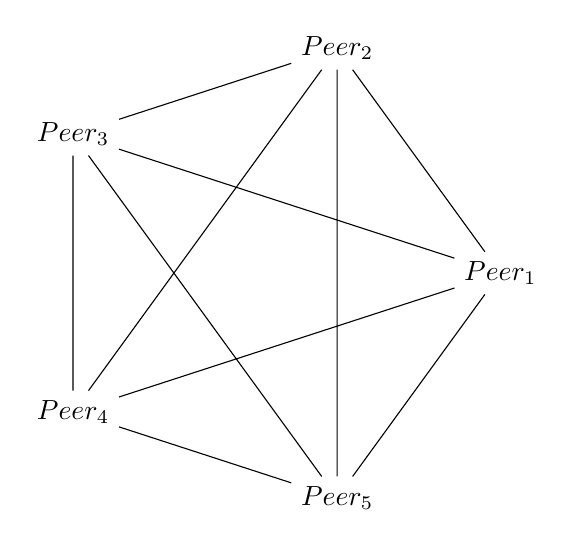
\begin{tikzpicture} [scale=1, transform shape]
%\tikzstyle{every node}=[draw,shape=circle];
\node (v1) at ( 0:3) {$Peer_1$};
\node (v2) at ( 72:3) {$Peer_2$};
\node (v3) at (2*72:3) {$Peer_3$};
\node (v4) at (3*72:3) {$Peer_4$};
\node (v5) at (4*72:3) {$Peer_5$};
\draw (v1) -- (v2) % fully connected
(v1) -- (v3)
(v1) -- (v4)
(v1) -- (v5)
(v2) -- (v3)
(v2) -- (v4)
(v2) -- (v5)
(v3) -- (v4)
(v3) -- (v5)
(v4) -- (v5);
\end{tikzpicture}
\caption{对等体架构}
\label{P2P}
\end{center}
\end{figure}

{\pa}的主要缺点在于一致性和可扩展性。为了保障一致性,{\pa}常常使用全相连网络(如图~\ref{P2P}),这样每个事件产生之后就可以同时发给所有对等体。然而,这种全相连网络的可扩展性是很差的。如果网络中有~$N$~个用户对一事件感兴趣,那么产生该事件的用户就要向网络中发出~$N$~条信息,网络中的通信量就会以玩家数量的平方数的速度增长。为了减少通信量,{\pa}常常需要依靠多播技术,然而多播技术在目前的因特网中并不普遍。幸运的是,{\pa}并不一定要使用全相连网络,许多文献中提到了用动态创建覆盖网络的方法来支持对等体间通信~\cite{p2p1, p2p2},这些方法提升了{\pa}的可扩展性。

另外,由于无法对用户产生的事件集中验证,在{\pa}中作弊会相对容易。

% . . . . . . . . . . . . . . . . . . . . . . . . . . . . . . . . %
\subsubsection{\da}
% 分布式架构  好处与缺点

{\da}可以看做{\csa}的进化版本。它与{\csa}类似的地方是它也拥有客户端(\ioc)和服务器(\gss)这样的分类,~\ioc~之间也不许直接连接,必须经过~\gss~中转。不过{\da}没有中央服务器,而是有分布的服务器群。游戏状态由这个群来管理。根据~\gss~组织方式的不同,{\da}又可以分为三类。

第一类:每个~\gss~维护一个游戏环节,每个~\ioc~只能连接到一个~\gss~并且只能与它交换数据。这类{\da}本质上就是多个{\csa}。它在一定程度上解决了游戏整体的可扩展性的问题,但是同时也限制了单个游戏环节的可扩展性。并且单点故障的问题仍然没有解决。

第二类:每个~\gss~维护游戏状态的一个子集。将游戏中的虚拟世界分块,每个~\gss~执掌一个块的游戏状态。~\ioc~根据其虚拟角色所在虚拟位置选择它要连接的~\gss。这样做可以显著地降低各个~\gss~的运算负担,但是同样无法解决单点故障问题。另外~\ioc~与~\gss~的连接方式会带来不公,且当虚拟角色在虚拟世界上发生大幅位移时还需要切换~\gss。

\begin{figure}[htbp]
\begin{center}
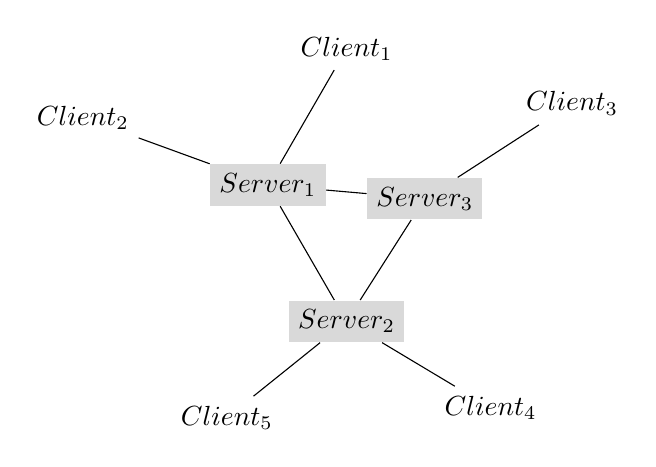
\begin{tikzpicture} [scale=1, transform shape]
%\tikzstyle{every node}=[draw];
\node [fill = gray!30] (s1) at (0:0) {$Server_1$};
\node [fill = gray!30] (s2) at (300:2) {$Server_2$};
\node [fill = gray!30] (s3) at (355:2) {$Server_3$};
\node (c1) at (60:2) {$Client_1$};
\node (c2) at (160:2.5) {$Client_2$};
\node (c3) at (15:4) {$Client_3$};
\node (c4) at (315:4) {$Client_4$};
\node (c5) at (260:3) {$Client_5$};
\draw (s1) -- (s2) -- (s3) -- (s1);
\draw (c1) -- (s1) -- (c2)
(c4) -- (s2) -- (c5)
(c3) -- (s3);
\end{tikzpicture}
\caption{分布式}
\label{distributed}
\end{center}
\end{figure}

第三类:每个~\gss~维护游戏状态的一个副本。这类结构又称“{\ma}”。每个~\ioc~连接到距离它较近的~\gss,并以客户~\slash~服务器的模式与它交换数据。~\gss~之间可以用等级化的方式组织,也可以用~P2P~的方式组织(如图~\ref{distributed})。

如果使用~P2P~形式组织~\gss,那么这种结构就比较稳健,且不存在中央瓶颈。但是它也会需要一个同步机制来保障多个~\gss~之间的一致性。由于{\ma}中的~\gss~数量通常少于{\pa}中的节点数,所以{\ma}中的同步相对容易一些。





%-------------------------------------------------%
\subsection{游戏架构的八项服务}
% 网络结构需要为游戏提供的八项服务(400字)
% 见意大利论文
\label{service}

一个完整的游戏架构不应当只是由~\ioc~和~\gss~两类实体堆砌而成,而应该能够提供以下八项服务~\cite{openping, dsl}:

\begin{description}
\item[状态维护(State Maintenance)]
GSS~维护游戏状态。这个游戏状态包括虚拟世界和这个世界中所有角色的状态。

\item[一致性维持(Consistency Maintenance)]
由于不同的用户拥有不同的延时,因此他们各自看到的虚拟世界可能存在时间上的冲突和差异,因此需要提供一致性维持服务来减小甚至消除此种差异。

\item[群组管理(Group Management)]
对用户分组以及事件过滤服务也很有用,因为并非所有用户都希望得到一样的信息,这与游戏本身的语义和玩家的运算能力都有关。

\item[事件通知(Event Delivery)]
所有玩家都拥有平等的被通知权。不应该因技术原因使玩家收到通知的时间和质量存在差异。

\item[账号与认证(Accounting, Authorization)]
有时在游戏开始之初用户可以选择环境和设定参数。游戏可以通过账号来认证用户。

\item[作弊控制(Cheating Control)]
玩家的动作必须经检验才可以向其他玩家通知。一些有趣的防止作弊的方法如~\cite{cheat1, cheat2, cheat3, cheat4}。

\item[玩家间通信(Player Communication)]
玩家间实时的文字、音频、视频通信可以增强用户体验。

\item[多媒体资料传播(Multimedia Resource Distribution)]
传统观点中多媒体资料的传播仅仅局限于游戏开始之前的“离线”下载阶段~\cite{traditional}。而新兴的观点则认为多媒体资料的下载将贯穿整个游戏过程,并增强用户间互动,提升游戏的可玩性~\cite{modern1, modern2, modern3}。
\end{description}
%-------------------------------------------------%

\subsection{一致性——同步的目的}
\label{def}
% 400字


%============================%

\section{传统~IP~网络中的经典同步机制}
\label{traditional}

\subsection{同步算法}
% 600字

\subsection{保守同步算法}

\subsection{优化同步算法}


%============================%

\section{新兴数据命名网络中的同步机制}
\label{innovative}
%(100字)

\subsection{CCN~中的~SYNC~协议}
% 800字

\subsection{用户自定义协议}
% 200字

\subsection{其它新型网络中的同步}
% 200字

\bibliography{data/zjubib}